% Appendix F

\chapter{Supplementary analysis} % Main appendix title
\chaptermark{Supplementary analysis}
\label{AppendixE} % For referencing this appendix elsewhere, use \ref{AppendixA}

%\lhead{Appendix C. \emph{Statistical Tests}} % This is for the header on each page - perhaps a shortened title

\section{Discovering phenotypic classes with unsupervised learning}

Whereas in the morphological screen most cells fall neatly into recognisable classes, our drug screen is more obscure. By inspection, the cell populations are dramatically less rich phenotypically than the morphological screen. There are many aberrant morphologies (see for example Figure \ref{fig:cell_crop_samples}) among the perturbed cell populations, but mitotic cells are scarce, and apoptotic cells are non-existent due to the washing of fluorescent dyes (and along with them, unfastened cells) prior to imaging. Machine learning is therefore an appropriate tool for wheedling out more subtle phenotypes.

We use clustering algorithms on the respective cell line datasets in an attempt to discover cell classes. To reduce dimensionality and to select between features with high mutual correlation between some of the extracted features\footnote{For example, many shape features extracted by Cell Cognition, such as area, perimeter, convex hull, will increase together.}, we apply principal components analysis (PCA). The large dataset remains restrictive in size to applying certain clustering algorithms. We therefore subsample the data. However, rather than uniform random sampling, we do the following: first, we apply k-means clustering to the dataset, choosing a potentially excessive number of clusters ($K = 30$). We expect this to identify small isolated clusters that may be lost by random sampling alone, as it is anticipated that interesting phentypes will be scarce. Then, we create a subsample of the dataset by sampling $50$ cells (where available) from each cluster. With this new, smaller dataset, we apply clustering algorithms robust to anisotropic data, including: DBSCAN (\cite{ester1996density}), spectral clustering (\cite{von2007tutorial}), and hierarchical clustering (\cite{ward1963hierarchical}). We visualise the outcomes of the clustering, choosing $K = 6$, as t-SNE embeddings in two dimensions in Figure \ref{fig:tnse_of_clusterings}.

\begin{figure}[h!]
\centering
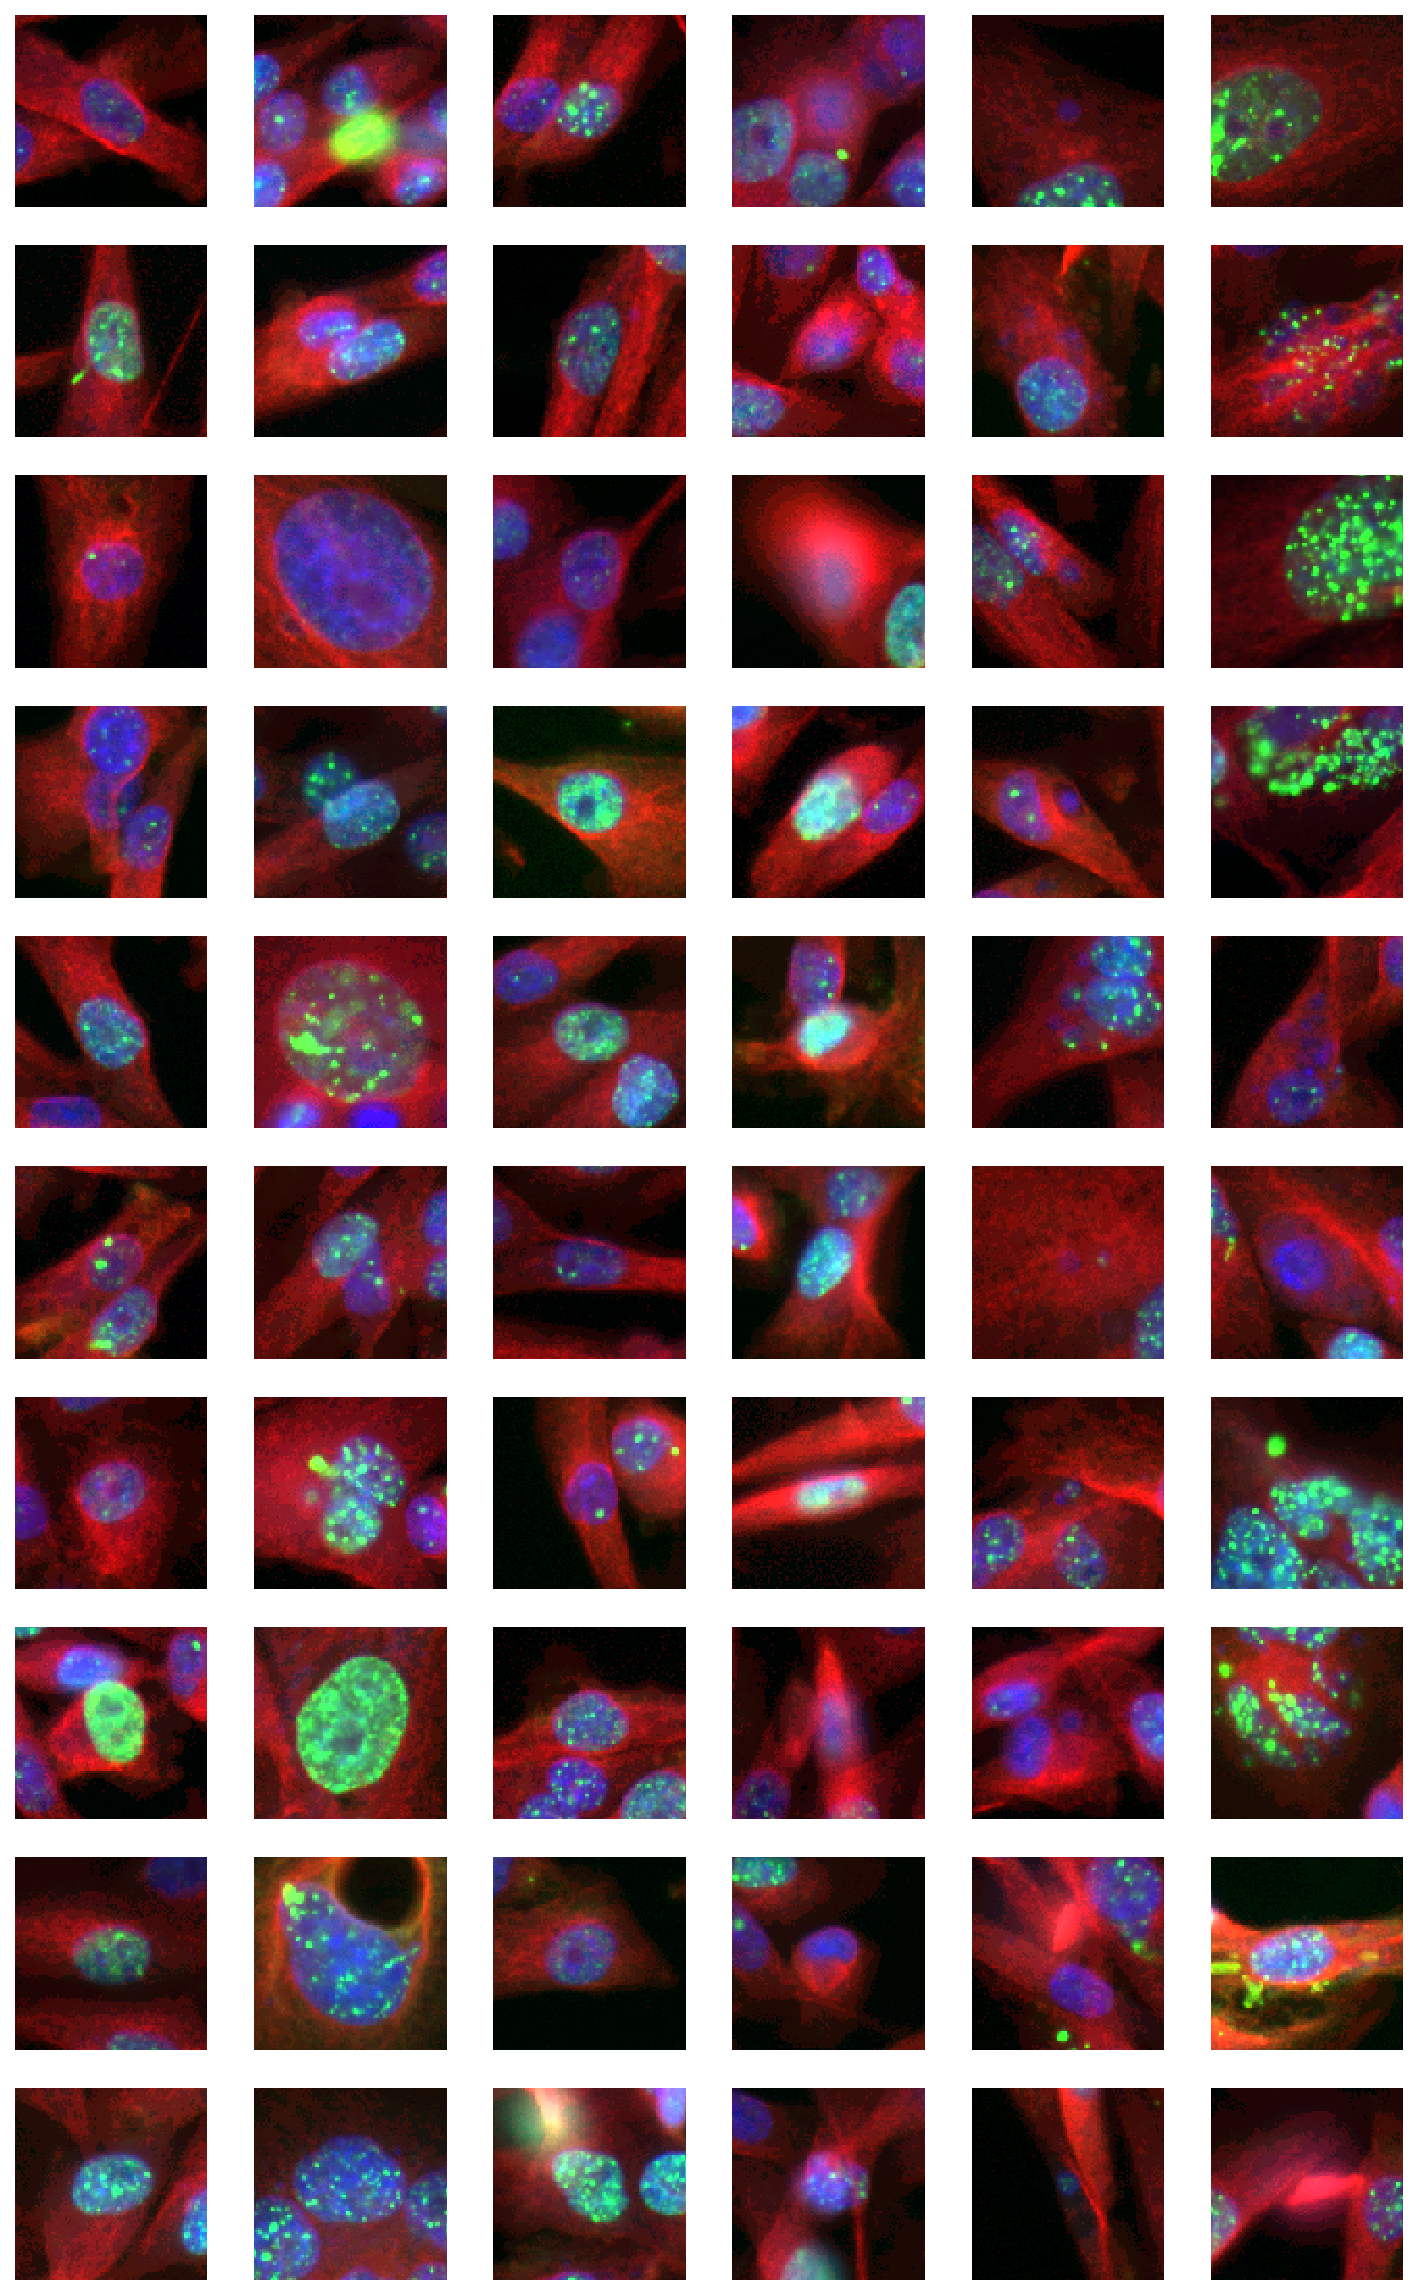
\includegraphics[width=0.95\textwidth]{img/samples.pdf}
\caption{Examples of spots (red) on cell nuclei detected with diameter openings on the Cy3 channel (grey).}
\label{fig:cell_crop_samples}
\end{figure}

%\begin{figure}%
%    \centering
%    \subfloat[Hierachical clustering]{{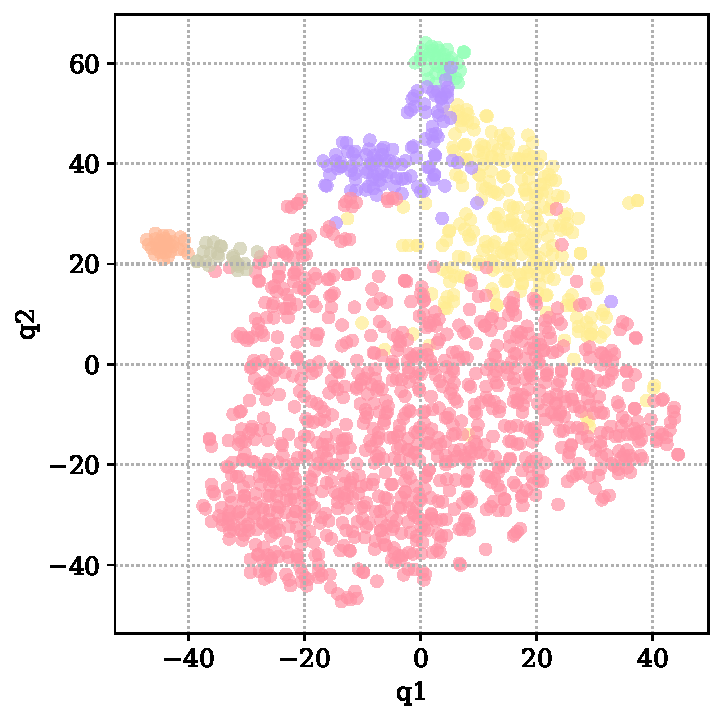
\includegraphics[width=0.45\textwidth]{img/clustering_hierarchical.pdf}}}
%    \qquad
%    \subfloat[Spectral clustering]{{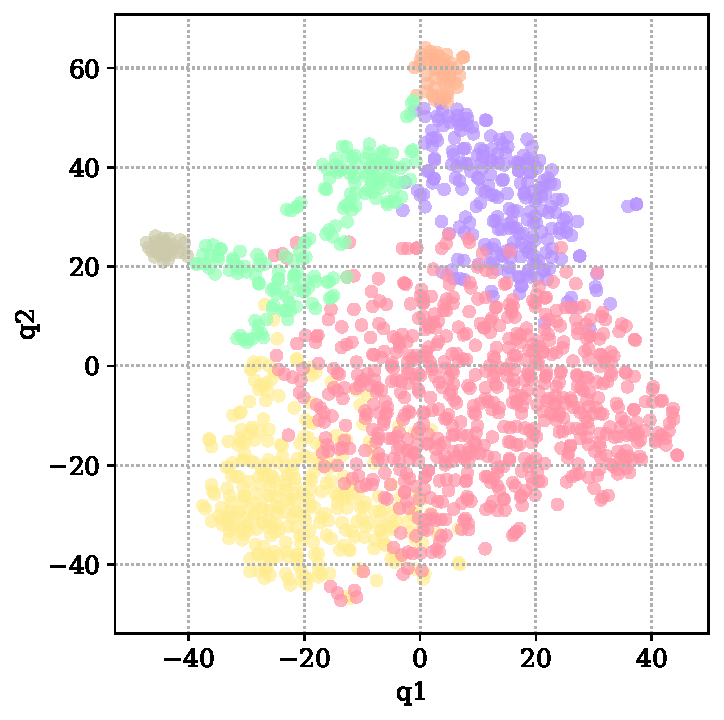
\includegraphics[width=0.45\textwidth]{img/clustering_spectral.pdf}}}
%    \caption{T-SNE plots of 1500 randomly sampled cells from clustering outcomes for hierachical clustering (a), and spectral clustering (b).}%
%    \label{fig:tnse_of_clusterings}%
%\end{figure}

We explore the clusters visually, by cropping examples of cells corresponding to each cluster. In Figure \ref{fig:cell_crop_samples} we see some subtle patterns emerge. The first cluster, the largest, appears to contain normal interphase cells. A second shows a mixture of normal and large interphase nuclei. Note that given our approach, it is anticipated that the predominant class, normal interphase, leaks into other clusters.   Elsewhere, we see a smaller cluster comprising of many micro-nucleated cells, and another containing cells with high levels of DNA damage.

The ultimate specification of morphological classes should be determined by domain experts, with unsupervised learning merely providing a starting point. After this, one could pursue an analysis such as in Section \ref{subsubsec:morphological_profile}. While we feel this is an interesting approach, we turn rather to fully unsupervised methods in Chapter \ref{Chapter3} to address the motivating questions of the assay.

\section{Training a RoI classifier}
\label{sec:training_roi_classifier}
We design a training set based on randomly placing $16$ randomly chosen $28 \times 28$px digits from the MNIST digits dataset on a $256 \times 256$ background ``canvas'' image as shown in Figure \ref{fig:roi_layers} (left).

\begin{figure}[h]
\centering
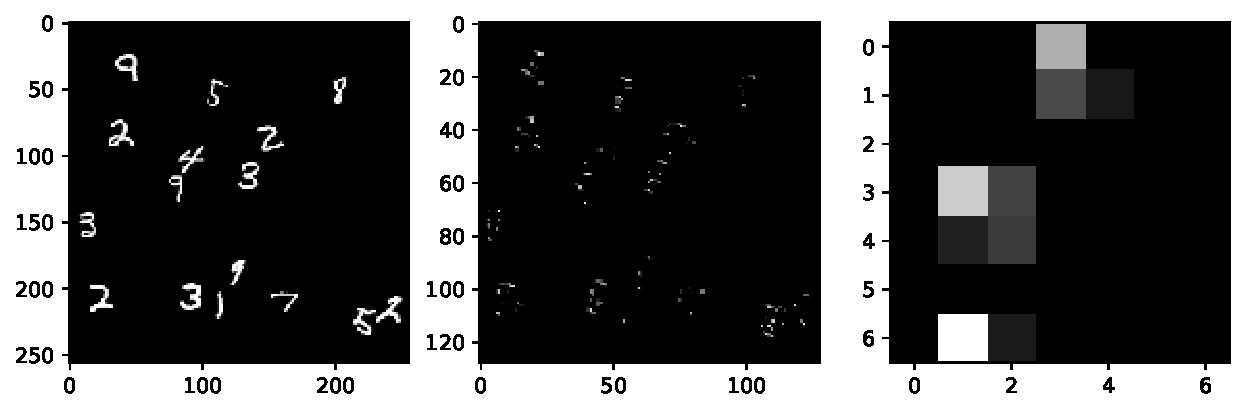
\includegraphics[width=0.95\textwidth]{img/roi_layers_full.pdf}
\caption{From left to right: canvas input, activation map after MaxPooling layer, activation map after RoIAlign layer (reduced to single bounding box).}
\label{fig:roi_layers}
\end{figure}

We implement an region of interest (RoI) classifer as a convolutional neural network $\texttt{Conv}_{1, 8} \rightarrow \texttt{ReLU} \rightarrow \texttt{MaxPool} \rightarrow \texttt{Conv}_{8, 16} \rightarrow \texttt{ReLU} \rightarrow \texttt{RoIAlign} \rightarrow \texttt{FC}_{784, 10}$, that is, a series of convolutional layers with ReLU activations followed by a RoIPool layer, and finally a fully-connected classification layer. The classifier is trained by a forward pass of such a canvas image, with the bounding box coordinates $(x_0, y_0, x_1, y_1)$ for each of the digits. According to the bounding boxes, the RoIAlign layer separates the image into a pseudo-batch of RoIs, which are subsequently classified into one of the $10$ digit classes by a softmax activation. Note that in this case, we choose the RoIAlign layer to quantise the incoming $14\times14$ tensors to $7\times7$ tensors. The stages of the forward pass are shown in Figure \ref{fig:roi_layers}. Trained in this manner, the classifier achieves $97\%$ accuracy as a classifier of MNIST digits, thus a small percentage shy of the accuracy of a typical MNIST classifier. In a single forward pass, the classifier can make predictions for the whole canvas, as illustrated in Figure \ref{fig:roi_prediction}. 

\begin{figure}[h]
\centering
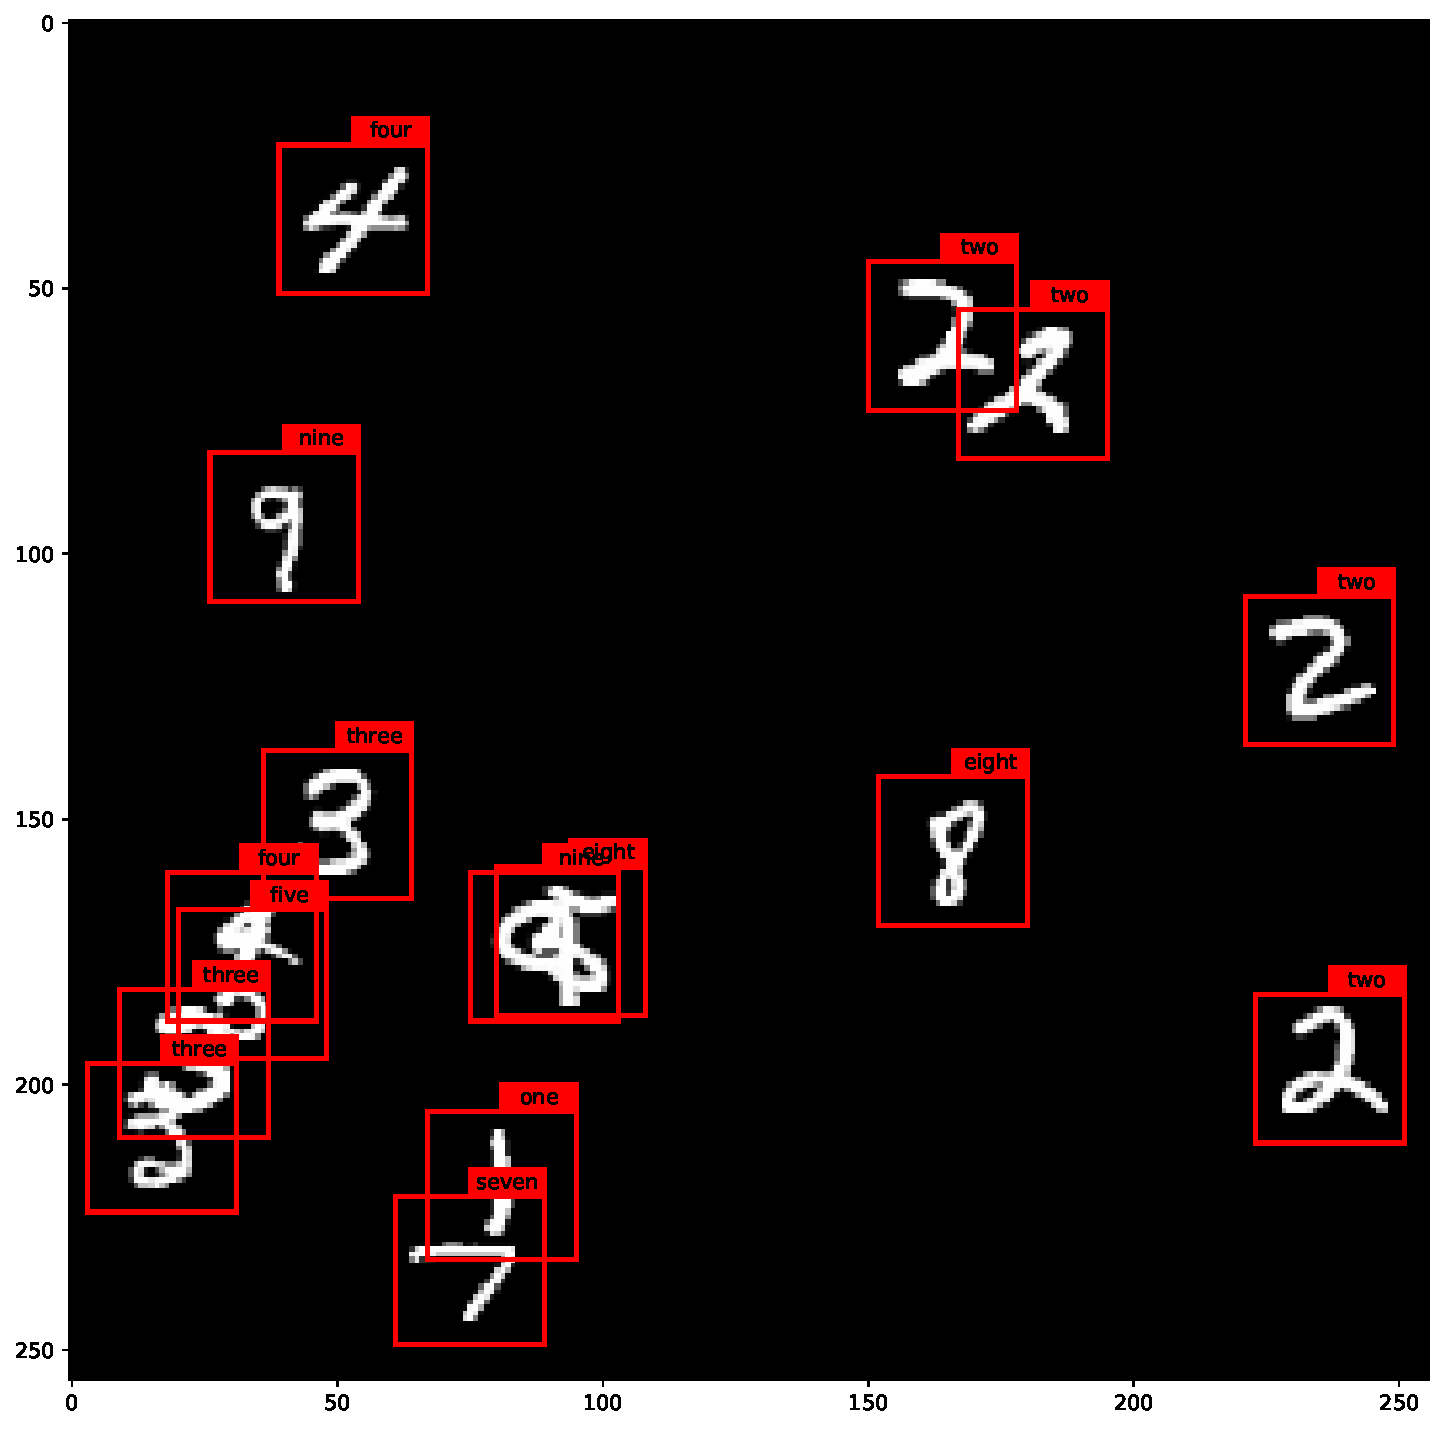
\includegraphics[width=0.95\textwidth]{img/roi_prediction.pdf}
\caption{Prediction of $16$ digits over canvas, performed in a single forward pass.}
\label{fig:roi_prediction}
\end{figure}

We can also incorporate our RoI classifier as a discriminator (that is, as a binary real/fake classifier) in conditional image-to-image GAN(\texttt{pix2pix}) framework. Now, in addition to an input canvas of MNIST digits, we create conditioning images for each class (here `0' or `1' digits). An example is given in Figure \ref{fig:roi_prediction}. We succeed in training a \texttt{pix2pix} system with a region of interest discriminator. We see in Figure \ref{fig:}. The \texttt{pix2pix} generator has thus learned to synthesis object detection images according to programmed localisation and classification information.

\begin{figure}[b!]
\centering
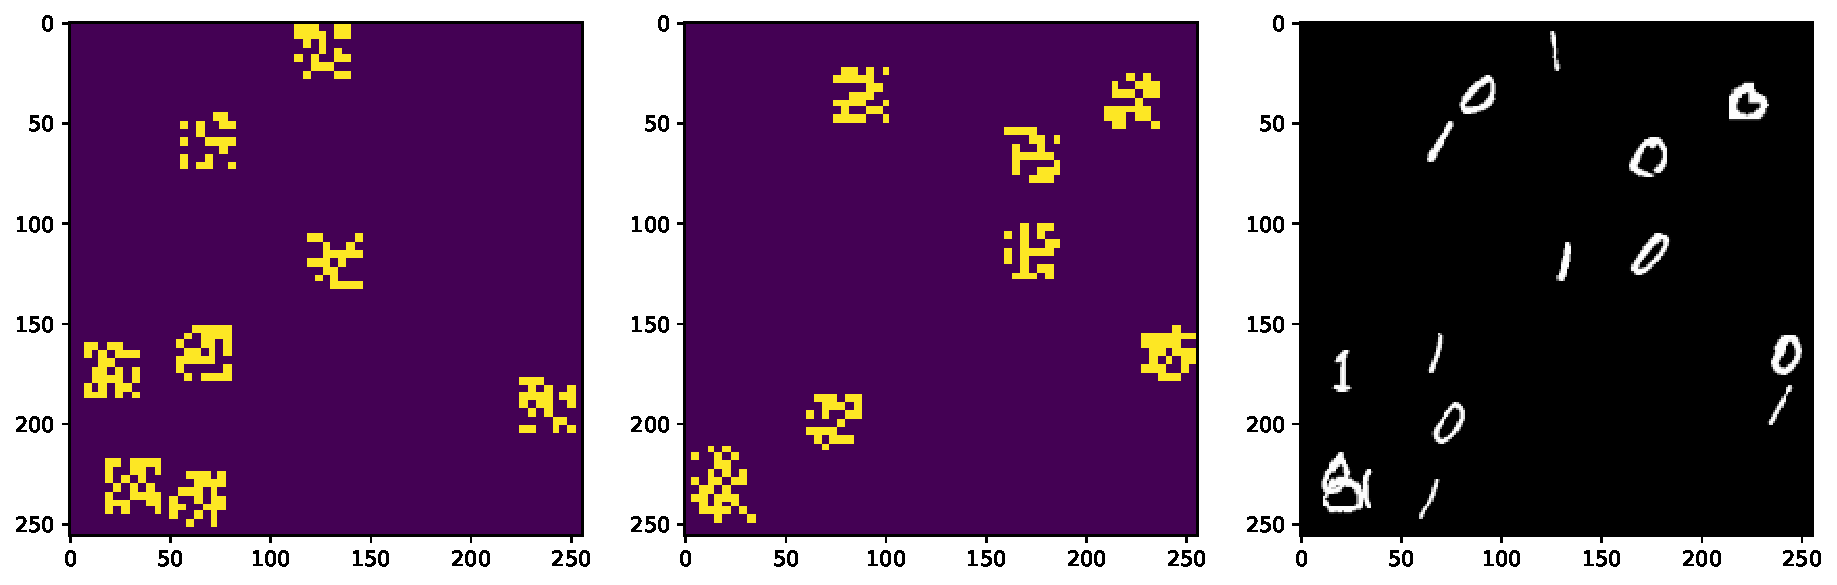
\includegraphics[width=0.95\textwidth]{img/roi_pix2pix_canvas.pdf}
\caption{Encodings of class and localisation specificiation (left and center) and corresponding train image for training conditional GAN with RoI discriminator.}
\label{fig:roi_prediction}
\end{figure}

In Figure \ref{fig:roi_mnist_comparison} we compare (using the same specification of object localisation and class) a ground truth image with that synthesised by a \texttt{pix2pix} system with our RoI discriminator and that with a plain \texttt{pix2pix} system. We see a far greater degree of mode collapse on the baseline compared with our proposed model.

\begin{figure}[h]%
    \centering
    \subfloat[Ground truth]{{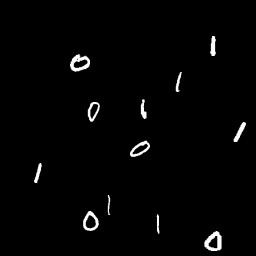
\includegraphics[width=0.3\textwidth]{img/roi_mnist_true.png} }}%
    \qquad
    \subfloat[\texttt{pix2pix}]{{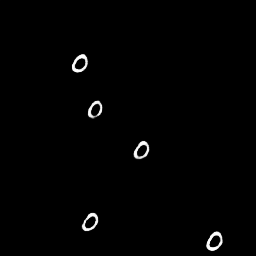
\includegraphics[width=0.3\textwidth]{img/roi_mnist_patch.png} }}%
    \subfloat[\texttt{pix2pix} + RoI discrimination]{{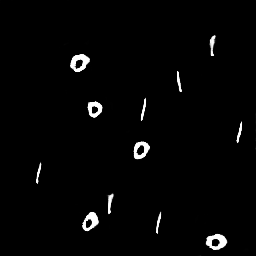
\includegraphics[width=0.3\textwidth]{img/roi_mnist_roi.png} }}%
    \qquad
    \caption{With the same specification of object localisation and class, a ground truth image (a), a synthetic image from a plain \texttt{pix2pix} system (b) and synthetic image from our \texttt{pix2pix} with RoI discrimination.}%
    \label{fig:roi_mnist_comparison}%
\end{figure}
